
\chapter{Reconstruction of Pt/Pd Bimetallic Near Surface Alloys Exposed to Carbon Monoxide}


\section{Introduction}


%intro line about catalysts
Catalysts are at the center of numerous industrial and scientific processes,
however the majority of effective catalysts are composed of expensive metals
such as \ce{Pt}, \ce{Pd}, \ce{Rh}, \ce{Au}, and \ce{Ag}.  In order to address
this issue of costly catalytic materials there has been an impetus to design
and characterize new bimetallic materials,\citep{Yu:2012by, Han:2015qr}
near-surface alloys (NSA),\citep{Jan-Kundsen:2007fe, Stephens:2011bv} and
dispersed nanostructures\citep{Shibata:2002hh,Kugai:2011rt} from cheaper
materials.  These catalysts have the potential to be finely-tuned for specific
reactions while reducing the needed amount of the expensive metal by replacing
it with a cheaper one. As an example \ce{Pt3Ni} catalysts have been created
that show an increased activity for the oxygen reduction reaction while
replacing a portion of \ce{Pt} with the much cheaper
\ce{Ni}.\cite{Stamenkovic:2007kk,Tuaev:2013fk} The stability of these types of
materials is called into question however as Tao {\em et al.} show in their
study of \ce{Pd/Rh} core-shell nanoparticles which experienced large-scale
inversions of material depending on the oxidizing or reducing nature of the
environment.\citep{Tao:2008aa} That is, under an oxidizing atmosphere, \ce{Rh}
made up the outer shell of the nanoparticle while under a reducing atmosphere,
\ce{Pd} migrated to the surface instead. This appendix provides information on
the initial creation of bimetallic Pt/Pd near-surface alloys and the
preliminary results obtained before the project was shelved.

\section{Methodology}
The (111) systems were initially thermalized at 200~K and warmed up in the
canonical (NVT) ensemble  to 1000~K over 500 ps. They were then allowed to
reach equilibrium at 1000~K over another 500 ps at which point they were dosed
with a sufficient quantity of Carbon Monoxide (\ce{CO}) to correspond to either
0, 0.25, or 0.5 monolayers (ML) of coverage. The systems were further
equilibrated in the NVT ensemble for 500 ps before switching to the
microcanonical (NVE) ensemble for 6 ns of data collection. The (100) systems
were treated identically except that they were warmed and equilibrated at 600~K
and kept at that temperature throughout the simulation.

\subsection{Interaction Parameters}
The interaction potentials provided in Michalka {\em et
al.}\citep{Michalka:2015aa} are used here unchanged. Important to note is that
the \ce{Pd\bond{-}CO} interaction is slightly stronger than the
\ce{Pt\bond{-}CO} interaction for this parameterization.

\subsection{System Details}
The systems were constructed from a FCC \ce{Pt} crystal that was ``sliced'' to
display either a (111) or (100) facet in the {\em z}-direction while being
periodic in the {\em x} and {\em y} directions. The bulk of the crystal was
kept as \ce{Pt} while one or two layers directly underneath the surface were
converted to \ce{Pd}. The ideal systems are highlighted in the top row of
Figure \ref{fig:biSystems}. The (111) systems have dimensions of
$71.41\times82.44\times100$ \AA\textsuperscript{3}, while the (100) systems are
$68.78\times68.78\times100$ \AA\textsuperscript{3}. \ce{Pd} was chosen as the
subsurface layer because of its stronger binding to \ce{CO}. During preliminary
simulations, a variety of possible systems that switched the order of the
metals or the number of layers at the surface or beneath the surface led to no
reconstruction because of a lack of any driving force.  However, when \ce{Pt}
is on the surface, there are two effects that lead to restructuring, \ce{Pt}'s
higher surface energy, {\em i.e.} desire to be in a bulk environment, and the
greater strength of the \ce{Pd\bond{-}CO} compared to the \ce{Pt\bond{-}CO}
interaction.

\begin{table}
  \caption{PT/PD NEAR SURFACE ALLOY SIZES AND COMPOSITION}
  \centering
  \begin{threeparttable}
  \begin{tabular}{ c ccc }
  \hline
  \hline
  \textbf{System} & \textbf{Pt} & \textbf{Pd} &  \textbf{(Pd/total)} \\
  \hline
  100-1Pt-1Pd & 7776 & 1296  & 0.143 \\
  100-1Pt-2Pd & 6480  & 2592  & 0.286 \\
  111-1Pt-1Pd & 10800  & 1800  & 0.143 \\
  111-1Pt-2Pd & 9000 & 3600  & 0.286 \\
  \hline
  \hline
  \end{tabular}
  \end{threeparttable}
\label{tab:systems}
\end{table}


\begin{landscape}
\begin{figure}[p!]
\centering
  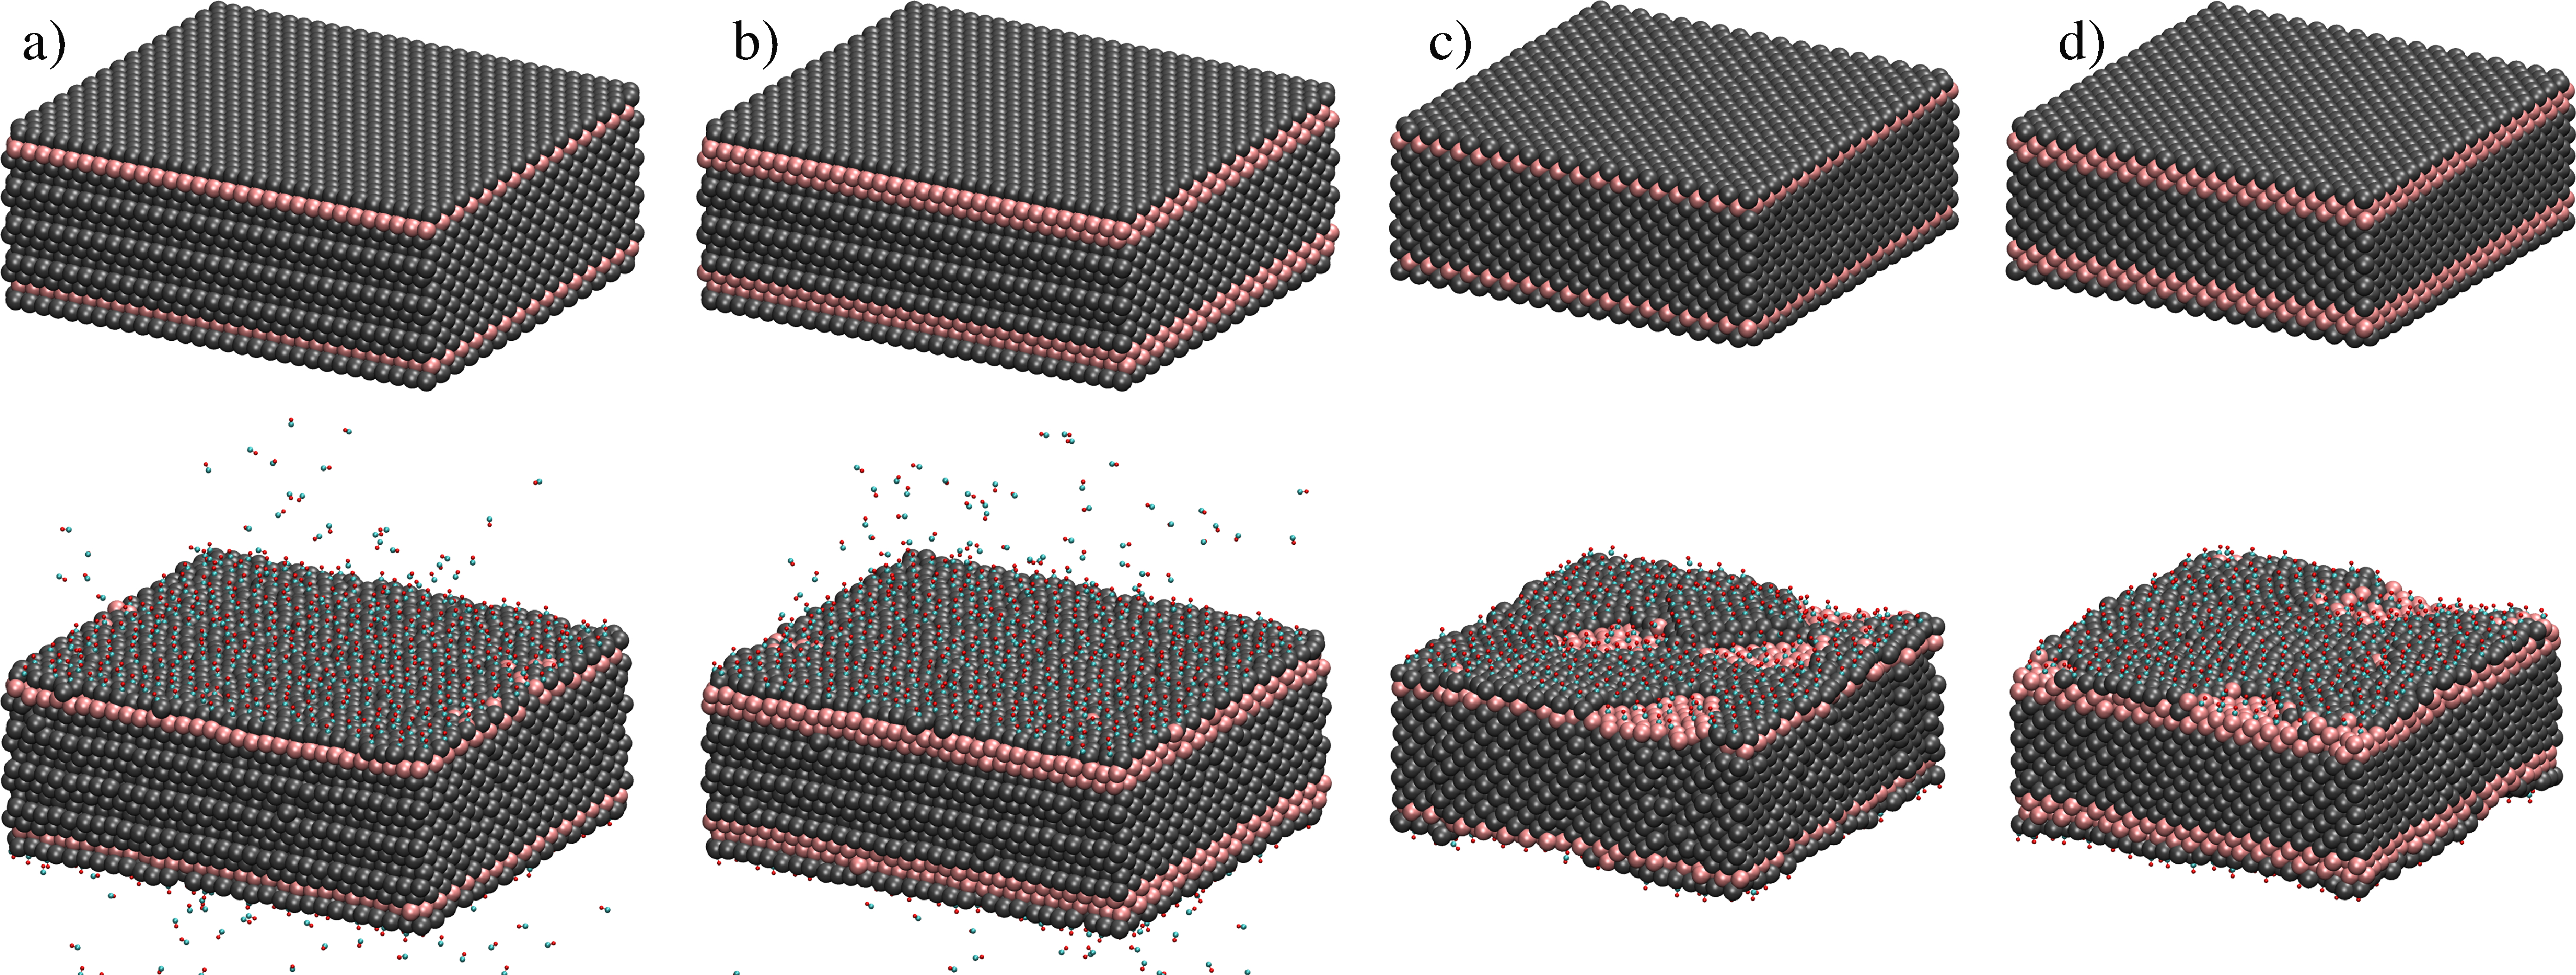
\includegraphics[width=0.8\linewidth]{../figures/appC/systems.pdf}
  \caption{Depictions of the (111) and (100) systems. \ce{Pt} atoms are colored
gray while \ce{Pd} are colored pink. The top row depicts near surface alloys
with a sandwiched Pt (surface), Pd (subsurface), Pt (bulk) system before
significant warming. Systems (a) and (b) display the low-energy (111) facets
and only differ with number of layers of Pd with (a) having one layer and (b)
having two layers. Systems (c) and (d) display the (100) facets on the surface
and also are only different with regard to the number of Pd layers, one and two
respectively.}
\label{fig:biSystems}
\end{figure}
\end{landscape}

\section{Results \& Discussion}
The (100) surfaces were inherently unstable at any CO-coverage and the surface
\ce{Pt} collapsed to domains of (111) which exposed the underlying (100)
\ce{Pd} which did remain fairly stable. As shown in Figure
\ref{fig:biSystems}.c and \ref{fig:biSystems}.d the initially (100) surface
restructures to the lower energy (111) domains. This is shown a bit more cleary
in Figure \ref{fig:surfaceGrid} although a small portion of the surface did
retain the original (100) motif. Additionally, because of the way adsorbate
coverage was initially calculated, this restructuring creates more surface
sites for the \ce{CO} to bind too which can be seen by comparing the (111) to
the (100) systems in Figure \ref{fig:biSystems} and seeing the large amount of
\ce{CO} that is not adsorbed in the (111) systems.

\subsection{Inversion}

\begin{figure}[p!]
\centering
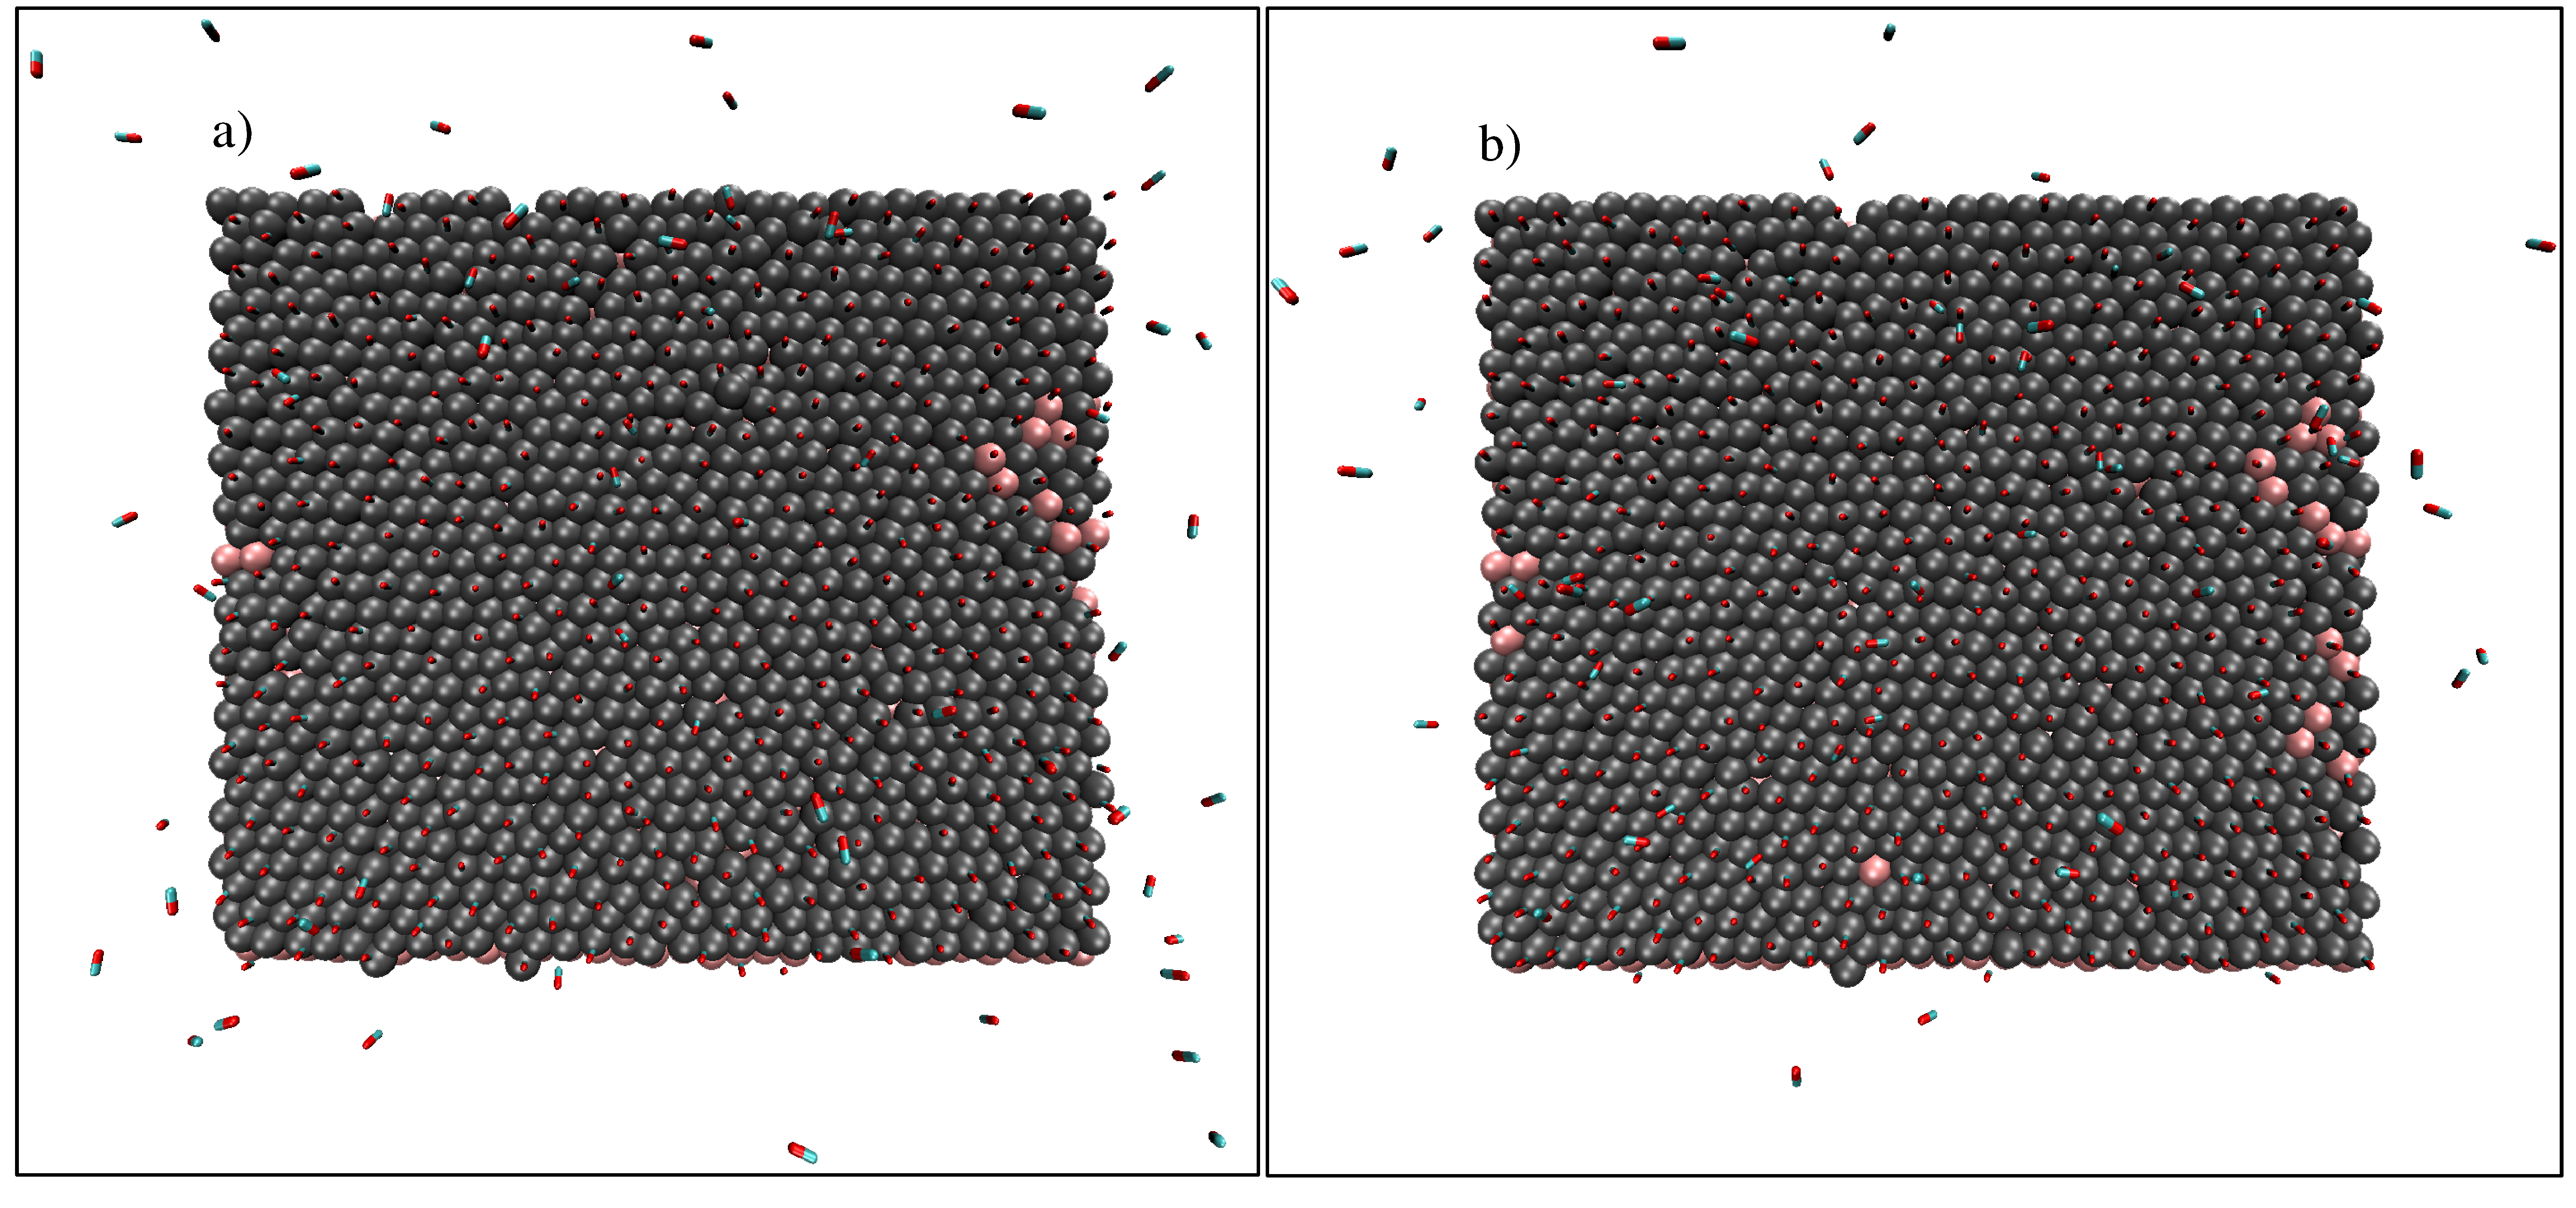
\includegraphics[width=\linewidth]{../figures/appC/inversion.pdf}
\caption{}
\label{fig:inversion}
\end{figure}
\end{landscape}

\subsection{Domain Formation}

\begin{landscape}
\begin{figure}[p!]
\centering
  \includegraphics[width=\linewidth]{../figures/appC/grid_small.pdf}
  \caption{Analysis of the roughened surface to find surface domain sizes was
carried out by mapping the surface composition (left) onto \AA\ spaced grid
points (center). Contiguous domains were identified and have been shown in
distinct colors (right), and the distribution of the domain areas was collected
over 15 ns time windows.}
\label{fig:surfaceGrid}
\end{figure}
\end{landscape}


\begin{figure}[p!]
\centering
  \includegraphics[width=\linewidth]{../figures/appC/ds_100_1Pt_2Pd_Pt.pdf}
  \caption{Distributions of Pt domain sizes at different CO coverages and at
different times after exposure to \ce{CO} for the 100-1\ce{Pt}-2\ce{Pd}
systems.}
\label{fig:ds100Pt}
\end{figure}


\begin{figure}[p!]
\centering
  \includegraphics[width=\linewidth]{../figures/appC/ds_100_1Pt_2Pd_Pd.pdf}
  \caption{Distributions of Pd domain sizes at different CO coverages and at
different times after exposure to \ce{CO} for the 100-1\ce{Pt}-2\ce{Pd}
systems.}
\label{fig:ds100Pt}
\end{figure}

\section{Summary}
The reconstruction that was observed on these systems was ultimately attributed
to the unstableness of the (100) surface facet rather than to any primarily
\ce{CO} induced effect. However, the presence of \ce{CO} did appear to
facilitate some of this reconstruction as shown in the domain plots and
inversion figures. Similar to what was seen in Chapter 3, the stronger
\ce{Pd\bond{-}CO} interaction coupled with the preference for \ce{Pt} to
maximize nearest neighbors provided the main driving force for these
reconstructions, but the presence of \ce{CO} also played a small role by
weakening the metal-metal bonds speeding up many of these processes. Future
simulations that ensure the stability of the bare surfaces may be able to speak
more clearly about the effects of \ce{CO} on these systems.

